This manuscript
(\href{https://lubianat.github.io/quali_phd/v/bdc5dbf4cb3698c1da65b9939fa935424b927361/}{permalink})
was automatically generated
from \href{https://github.com/lubianat/quali_phd/tree/bdc5dbf4cb3698c1da65b9939fa935424b927361}{lubianat/quali\_phd@bdc5dbf}
on December 9, 2021.

\hypertarget{authors}{%
\subsection{Authors}\label{authors}}

\begin{itemize}
\tightlist
\item
  \textbf{Tiago Lubiana}
  
\includegraphics{images/orcid.svg}
  \href{https://orcid.org/0000-0003-2473-2313}{0000-0003-2473-2313}
  · 
\includegraphics{images/github.svg}
  \href{https://github.com/lubianat}{lubianat}
  · 
\includegraphics{images/twitter.svg}
  \href{https://twitter.com/lubianat}{lubianat}
  School of Pharmaceutical Sciences, University of São Paulo; Ronin Institute
  · Funded by Grant \#2019/26284-1 from the São Paulo Research Foundation (FAPESP).
\end{itemize}

\hypertarget{abstract}{%
\section{Abstract}\label{abstract}}

The Human Cell Atlas (HCA) is an international effort aiming at characterizing every cell type of the human body.
By techniques such as single-cell RNA sequencing, mass cytometry, and multiplexed in situ hybridization, HCA members are producing cell-level data from virtually all human tissues.
This wealth of data can significantly impact biomedical research, but only if its content is genuinely interoperable.
While ontologies and semantic technologies have emerged as key players in the data interoperability ecosystem, there are still gaps to cover between the technical possibilities and the practical applications in biomedical research.
In addition to ontologies, like the Cell Ontology and the Gene Ontology, large-scale knowledge graphs are growing as knowledge management tools.
Among those, Wikidata, a sister project of Wikipedia for structured data, is surfacing as a hub in the semantic web for multiple types of information.
The formatting and deployment of information from the Human Cell Atlas to Wikidata can increase information availability and impact, connecting the scientific products with the larger knowledge ecosystem.
This PhD project aims at studying Wikidata as a platform for representing cell types, addressing theoretical and practical concerns.\\
We review the literature on cell types, refining and formalizing concepts for cell type delimitation.
At the same time, we are enriching Wikidata with new classes curated from the literature and with large scale integrations of biomedical databases (e.g.~PanglaoDB) into the Wikidata infrastructure.
To aid that effort, we are developing Wikidata Bib, a framework for literature management and organized note-taking system for reading the academic literature with high efficiency.
Finally, we plan to improve the interplay of Wikidata, the Cell Ontology and software used for single-cell RNA-seq data, inserting Wikidata \emph{de facto} as a tool for the Human Cell Atlas community.

Here we present an overview of the different chapters that compose this document, presented as the text for a qualifying exam.\\
This work is concerned with the conceptual modelling of knowledge about cell types.
The introduction contains an overview of the Human Cell Atlas project and the current state of classifying cells into types.
Then, it proceeds to introduce ontologies and knowledge graphs as tools for connecting what we know about cells.

The methodology section is an overview of the core methods used throughout the work.
However, as the project contains elements from different scientific traditions, the results chapters might also display particular methods used in the specific branch of the project.

It is worth noticing that the different results shown were not developed chronologically in the order shown.
They were actually developed in parallel, with overlapping periods of activity.
They have been organized into separate chapters, however, as they tackle different perspectives of the subject matter and are part of different publications.

The discussion on the concept of cell type is presented first, as it is instrumental for the later steps.
It is followed by an account of how PanglaoDB, a database of cell markers, was integrated into Wikidata, based on a notion of species-specific cell type clarified in the preceding chapter.

Then, we present Wikidata Bib, a framework for an organized reading of the literature.
The framework, although used as a method throughout the PhD project, is presented in the results session.
We emphasize the technical and theoretical details of the system are part of the intellectual work put into the project.
The system evolved into a biocuration platform for the collection of cell types from the literature to Wikidata.
To end the results, we discuss how our efforts integrate with the Cell Ontology, the currently leading system for organizing cell types.

Finally, an account of other academic aspects of the project is presented as part of the qualification requirements.
They present an overview of collaborations, participation in events and academic courses taken during the first part of the PhD project.

\hypertarget{background}{%
\section{Background}\label{background}}

\hypertarget{the-human-cell-atlas-hca-project}{%
\subsection{The Human Cell Atlas (HCA) Project}\label{the-human-cell-atlas-hca-project}}

The advent of single-cell technologies has ignited the desire for a deep knowledge of cells, the building blocks of life {[}\protect\hyperlink{ref-pNGap1Du}{1}{]}.
The Human Cell Atlas (HCA) project has been a major player in the cell knowledge ecosystem, running since 2017 to characterize every cell type in the human body {[}\protect\hyperlink{ref-1GmbExweg}{2}{]}.
The HCA consortium gathers people from all over the world to tackle different parts of the project to have a diverse and equitable account of the cell type diversity. {[}\protect\hyperlink{ref-tjdjR2Xf}{3}{]}

Building a complete atlas of human cells comes with multiple challenges. The project includes the detection, in single cells, of RNA species (scRNA-Seq), chromatin accessibility (scATAC-Seq), and protein markers (primarily by CYTOF), as well as spatial information on cells with multiplexed \emph{in situ} hybridization (such as MERFISH) and imaging mass cytometry {[}\protect\hyperlink{ref-1GmbExweg}{2},\protect\hyperlink{ref-kkwRTArg}{4}{]}. Every lab inside the project will contribute with its expertise, providing samples representing human diversity.

HCA is set to revolutionize the biomedical sciences by creating tools and standards for basic research, allowing better characterization of disease, and improving diagnostics and therapy.
Its products (data, information, knowledge and wisdom) need to be FAIR: findable, accessible, interoperable and reusable.
Data stewardship and management are growing as core demands of the scientific community, ranging from data management plans {[}\protect\hyperlink{ref-1DSEIjFha}{5}{]} to specialized data personnel {[}\protect\hyperlink{ref-1DSEIjFha}{5}{]}.

The Human Cell Atlas has a dedicated team for organizing data: the Data Coordination Platform (DCP) {[}\protect\hyperlink{ref-zDRzmIGu}{6}{]} {[}\protect\hyperlink{ref-kkwRTArg}{4}{]}.
The DCP is responsible for tracing the plan for computational interoperability, from the data generators to the consumers.{[}\protect\hyperlink{ref-kkwRTArg}{4}{]}.
The Human Cell Atlas has its portal for data {[}\protect\hyperlink{ref-kX6KnbUo}{7}{]}), which composes the data repository landscape with other resources, like the Broad Institute Single Cell Portal {[}https://singlecell.broadinstitute.org/single\_cell\textgreater) and the Chan-Zuckerberg Biohub Tabula Sapiens (\url{https://tabula-sapiens-portal.ds.czbiohub.org/}).
In addition to its core team, the HCA is poised to grow by community interaction. It states in its opening paper that ``As with the Human Genome Project, a robust plan will best emerge from wide-ranging scientific discussions and careful planning''.{[}\protect\hyperlink{ref-1GmbExweg}{2}{]}\\
Thus, this project inserts itself among the wide-ranging scientific discussions to improve data - and knowledge - interoperability. {]})
The work also paves the way for Wikidata reconciling of other databases for cell-type markers, such as CellMarker {[}\protect\hyperlink{ref-chGii6yw}{8}{]}, labome {[}\protect\hyperlink{ref-rhRRCtlA}{9}{]}, CellFinder {[}\protect\hyperlink{ref-4AEy2xhQ}{10}{]} and SHOGoiN/CELLPEDIA {[}\protect\hyperlink{ref-6uWWsiSq}{11}/{]}) (if proper authorization are given by the owners).
The approach we took here can in essence be applied to any knowledge set of public interest, providing a low-cost and low-barrier platform for sharing biocurated knowledge in gold standard format.

\hypertarget{wikidata-bib-and-a-professional-system-for-biocuration}{%
\subsection{Wikidata Bib and a professional system for biocuration}\label{wikidata-bib-and-a-professional-system-for-biocuration}}

\hypertarget{introduction}{%
\subsubsection{Introduction}\label{introduction}}

Reading scientific articles is an integral part of the routine of modern scientists.
Although a number of literature/reference management software are available {[}\protect\hyperlink{ref-wikidata:https:ux2fux2fen.wikipedia.orgux2fwikiux2fComparison_of_reference_management_software}{\textbf{wikidata:https://en.wikipedia.org/wiki/Comparison\_of\_reference\_management\_software?}}{]}, the process of reading is largely artisanal.
There are no standard guidelines on how to probe the literature organize notes for biomedical researchers.
Thus, while reading and studying is a core activity, there are few (if any) protocols for efficient screening of scientific articles.

Other professional traditions have dealt with similar issues in the past.
In the field of accounting, note-taking is of outstanding importance, to keep track of financial balances and avoid costly problems.
Double-entry bookkeeping was developed in the 13th century as a professional solution for note-taking in accounting where ``every entry to an account requires a corresponding and opposite entry to a different account.'' {[}\protect\hyperlink{ref-uYuz0opI}{12}, =Double-entry\_bookkeeping\&oldid=1055066428{]}
In software development, Test-Driven Development (TDD) is a popular methodology where tests for code snippets are written before the code itself, therefore ensuring that written software passes minimum quality standards.
The similarities of Double-entry bookkeeping and TDD are diverse {[}\protect\hyperlink{ref-wikidata:https:ux2fux2fblog.cleancoder.comux2funcle-bobux2f2017ux2f12ux2f18ux2fExcuses.html}{\textbf{wikidata:https://blog.cleancoder.com/uncle-bob/2017/12/18/Excuses.html?}}{]}, but for our purpose here suffices to see both as professionalized systems that promote better quality and accountability of works.

In the humanities, there is a well-established practice of annotations of readings.
The annotation skills are part of common academic training in the humanities {[}\protect\hyperlink{ref-rPKBwmYh}{13}/{]}{[}\protect\hyperlink{ref-PKhuVRW8}{14}\_da26C-QW5qiS7uZ{]}.
An influential work in presenting methods for academic reading in the humanities is Umberto Eco's book ``How to Write a Thesis'' {[}\protect\hyperlink{ref-1HBVPtZGp}{15}{]}, which outlines not only \emph{how} to annotate the literature that basis an academic thesis, but also \emph{why} to do so.
The book, written originally in 1977, is still influential today, but its theoretical scope (roughly the humanities) and its date, preceding the digital era, limits the extent in which it applies to the biomedical sciences.

Notably, the need of an organized reading system for biocuration studies stems from a difference in methodology.
In humanities, the main (if not sole) research material is the written text, the books and articles from which research stems. {[}\protect\hyperlink{ref-PKhuVRW8}{14}\_da26C-QW5qiS7uZ{]}.
In the biomedical sciences, including a large part of bioinformatics, the object of study is the natural world, observed via experimentation.
Thus, naturally, scientific training focuses on the theoretical and practical basis of experimentation and data analysis.
With the bloom of scientific articles, however, the scientific literature (and accompaning public datasets) provide already a strong material for the sculpting of scientific projects.
Thus, the development of a methodology for academic reading, tailored to the digital environment, presents itself as a need.

This chapter concerns itself with presenting Wikidata Bib, a framework for large scale reading of scientific articles.
It is presented as three parts, each of them with a technical overview alongside the theoretical foundations.
First, Wikidata Bib is presenting as a reading system, for managing references and notes using a GitHub repository and plain text notes.
Then, we present how the system ensures accountability, allowing its user to get personalized analytics on their reading patterns.
Finally, we demonstrate how Wikidata Bib fits an active curation environment, connecting the framework with the larger goal of this project of curating information about cell types on Wikidata.

\hypertarget{wikidata-bib-as-a-reading-system}{%
\subsection{Wikidata Bib as a reading system}\label{wikidata-bib-as-a-reading-system}}

The reading framework of Wikidata bib is built upon a git repository integrated with GitHub, Python3 scripts and SPARQL queries.
It has a standard file structure, summarized as the following:

\begin{itemize}
\tightlist
\item
  \texttt{docs/}

  \begin{itemize}
  \tightlist
  \item
    \texttt{index.html}
  \end{itemize}
\item
  \texttt{downloads/}

  \begin{itemize}
  \tightlist
  \item
    \texttt{10.7554\_ELIFE.52614.pdf}
  \end{itemize}
\item
  \texttt{notes/}

  \begin{itemize}
  \tightlist
  \item
    \texttt{Q87830400.md}
  \end{itemize}
\item
  \texttt{src/}

  \begin{itemize}
  \tightlist
  \item
    \texttt{get\_pdf.py}
  \item
    \texttt{helper.py}
  \item
    \texttt{read\_paper.py}
  \item
    \texttt{update\_dashboard.py}
  \end{itemize}
\item
  \texttt{index.md}
\item
  \texttt{toread.md}
\item
  \texttt{config.yaml}
\item
  \texttt{pop}
\item
  \texttt{wadd}
\item
  \texttt{wadd\_all}
\item
  \texttt{wread}
\item
  \texttt{wlog}
\end{itemize}

The \texttt{docs/} directory contains the live dashboard from the readings, which will be discussed in the following sessions.
The \texttt{downloads/} directory hosts the pdfs of the articles read with the system.
These are not commited to the repository, and are only stored locally.
The \texttt{notes/} directory contains markdown files, one for each article read.
The \texttt{src/} directory contains the python code with the mechanics of the system.
They contain helper functions for the command line commands discussed below:
- \texttt{wread} which receives a Wikidata QID for an article and outputs (1) a notes document, (2) a pdf for the paper obtained from Unpaywall {[}\protect\hyperlink{ref-15luL9zZC}{16}/{]} and (3) an updated version of the dashboard html files in the \texttt{docs/} directory.
- \texttt{pop}, which ``pops'' an article from \texttt{toread.md} and runs \texttt{wread} for it
- \texttt{wadd}, which takes an URL for an Wikidata SPARQL query and adds new QIDs to \texttt{toread.md}
- \texttt{wadd\_all}, which parses \texttt{config.yaml} for recurrent SPARQL queries and runs \texttt{wadd} for each
- \texttt{wlog}, which adds, commits and pushes recent readings and dashboard updates to GitHub

All the structures described so far are commonly shared by any user of Wikidata Bib.
To personalize the use of the system, the user edits three plain text files.
\texttt{toread.md} hosts a plain text QIDs of the articles that will be read.
These can be added either manually, or via wadd.
While the \texttt{pop} command only sees QIDs, articles titles or other identifiers can be added to \texttt{toread.md} temporarily without breaking the system.
\texttt{index.md} hosts a numbered list of topics of interest.
This file plays the role of Umberto Eco's work plan, with the topics of interest for the academic. {[}\protect\hyperlink{ref-1HBVPtZGp}{15}{]}
These are used to tag articles for retrieval in a later step.
\texttt{config.yaml} contains shortcuts for different reading lists.
This is better explained by example.
In my \texttt{toread.md} file there are two reading lists, one following a \texttt{\#\ Cell\ types} header, and another following a \texttt{\#\ Biocuration} header.
My \texttt{config.yaml} contains the following snippet:

\begin{Shaded}
\begin{Highlighting}[]
\FunctionTok{lists}\KeywordTok{:}
\CommentTok{\# {-} shortcut: Title of header in toread.md  }
\AttributeTok{  }\FunctionTok{ct}\KeywordTok{:}\AttributeTok{ Cell types}
\AttributeTok{  }\FunctionTok{bioc}\KeywordTok{:}\AttributeTok{ Biocuration}
\end{Highlighting}
\end{Shaded}

The shortcuts in \texttt{config.yaml} are used as arguments by the \texttt{pop} command, where \texttt{\$\ ./pop\ ct} retrieves an article from the ``Cell types'' list, while \texttt{\$\ ./pop\ bioc} retrieves an article from the ``Biocuration'' list.

The Wikidata bib framework is coupled with a discipline of daily reading.
This is inspired by Robert Cecil Martin's description of Test Driven Development in the book ``Clean Code'', which includes not only a technical description, but a \emph{school of thought} of how software development can be approached. {[}\protect\hyperlink{ref-13HqB23xH}{17}{]}
Every day, I read one article of each list, using the notetaking station displayed in Figure \ref{fig:notetaking}.
The constancy of reading allows steady coverage of the relevant literature.
While it has worked for this research project, however, it is not required for use of the Wikidata Bib system.

The notetaking station of Wikidata Bib is, by default, opened in Virtual Studio Code, and is depicted on Figure \ref{fig:notetaking} A.
The title and publication dates are displayed, and the reading process entails copying snippets from the text to the ``Highlights'' session.
By copying the highlights into plain text, the sections of interest become searchable via command line using \texttt{grep} (https://en.wikipedia.org/w/index.php?title=Grep\&oldid=1039541979).
Comments can be added either in the comment section or inline, alongside the highlights, using \texttt{-\/-\textgreater{}\ Comment\ goes\ here} to differentiate from highlights.
Also searchable by \texttt{grep} are the tags, copied and pasted from \texttt{index.md} in the \texttt{\#\#\ Tags} session or alongside the main article.

The discipline also includes, whenever possible, an improvement of the metadata about the article on Wikidata.
In \ref{fig:notetaking} B are shown the links included in the dashboard.
A link to a Scholia {[}\protect\hyperlink{ref-hxzL9pmm}{18}{]} profile allows identification of related articles from a series of pre-made SPARQL queries probing bibliography data on Wikidata.
While Scholia provides an overview of a given article, it does not allow direct curation of the metadata.
For that, two links are provided, one to Wikidata and one to Author Disambiguator {[}\protect\hyperlink{ref-1A9RvszKC}{19}{]}.
By acessing the Wikidata page for the entity, one can add new triples, for example curating authors and topics of the article, which are then used by Scholia and by Wikidata Bib's dashboard.
Author Disambiguator is a wrapper of an Wikimedia API which facilitates the process of disambiguating author names to unique identifiers on Wikidata, thus feeding the publict knowledge graph of publication and authors.\\
Finally, a link to the article's DOI or full text URL is provided, and serves as a fallback when the automatic download fails.
Of note, while the metadata curation has a technical benefit to Wikidata and the dashboard, it also plays a theoretical role.
By curating metadata on authors, the user of Wikidata Bib can better understand the people they read, and expand their metascientific perspective on their domain of interest.

\begin{figure}
\hypertarget{fig:notetaking}{%
\centering
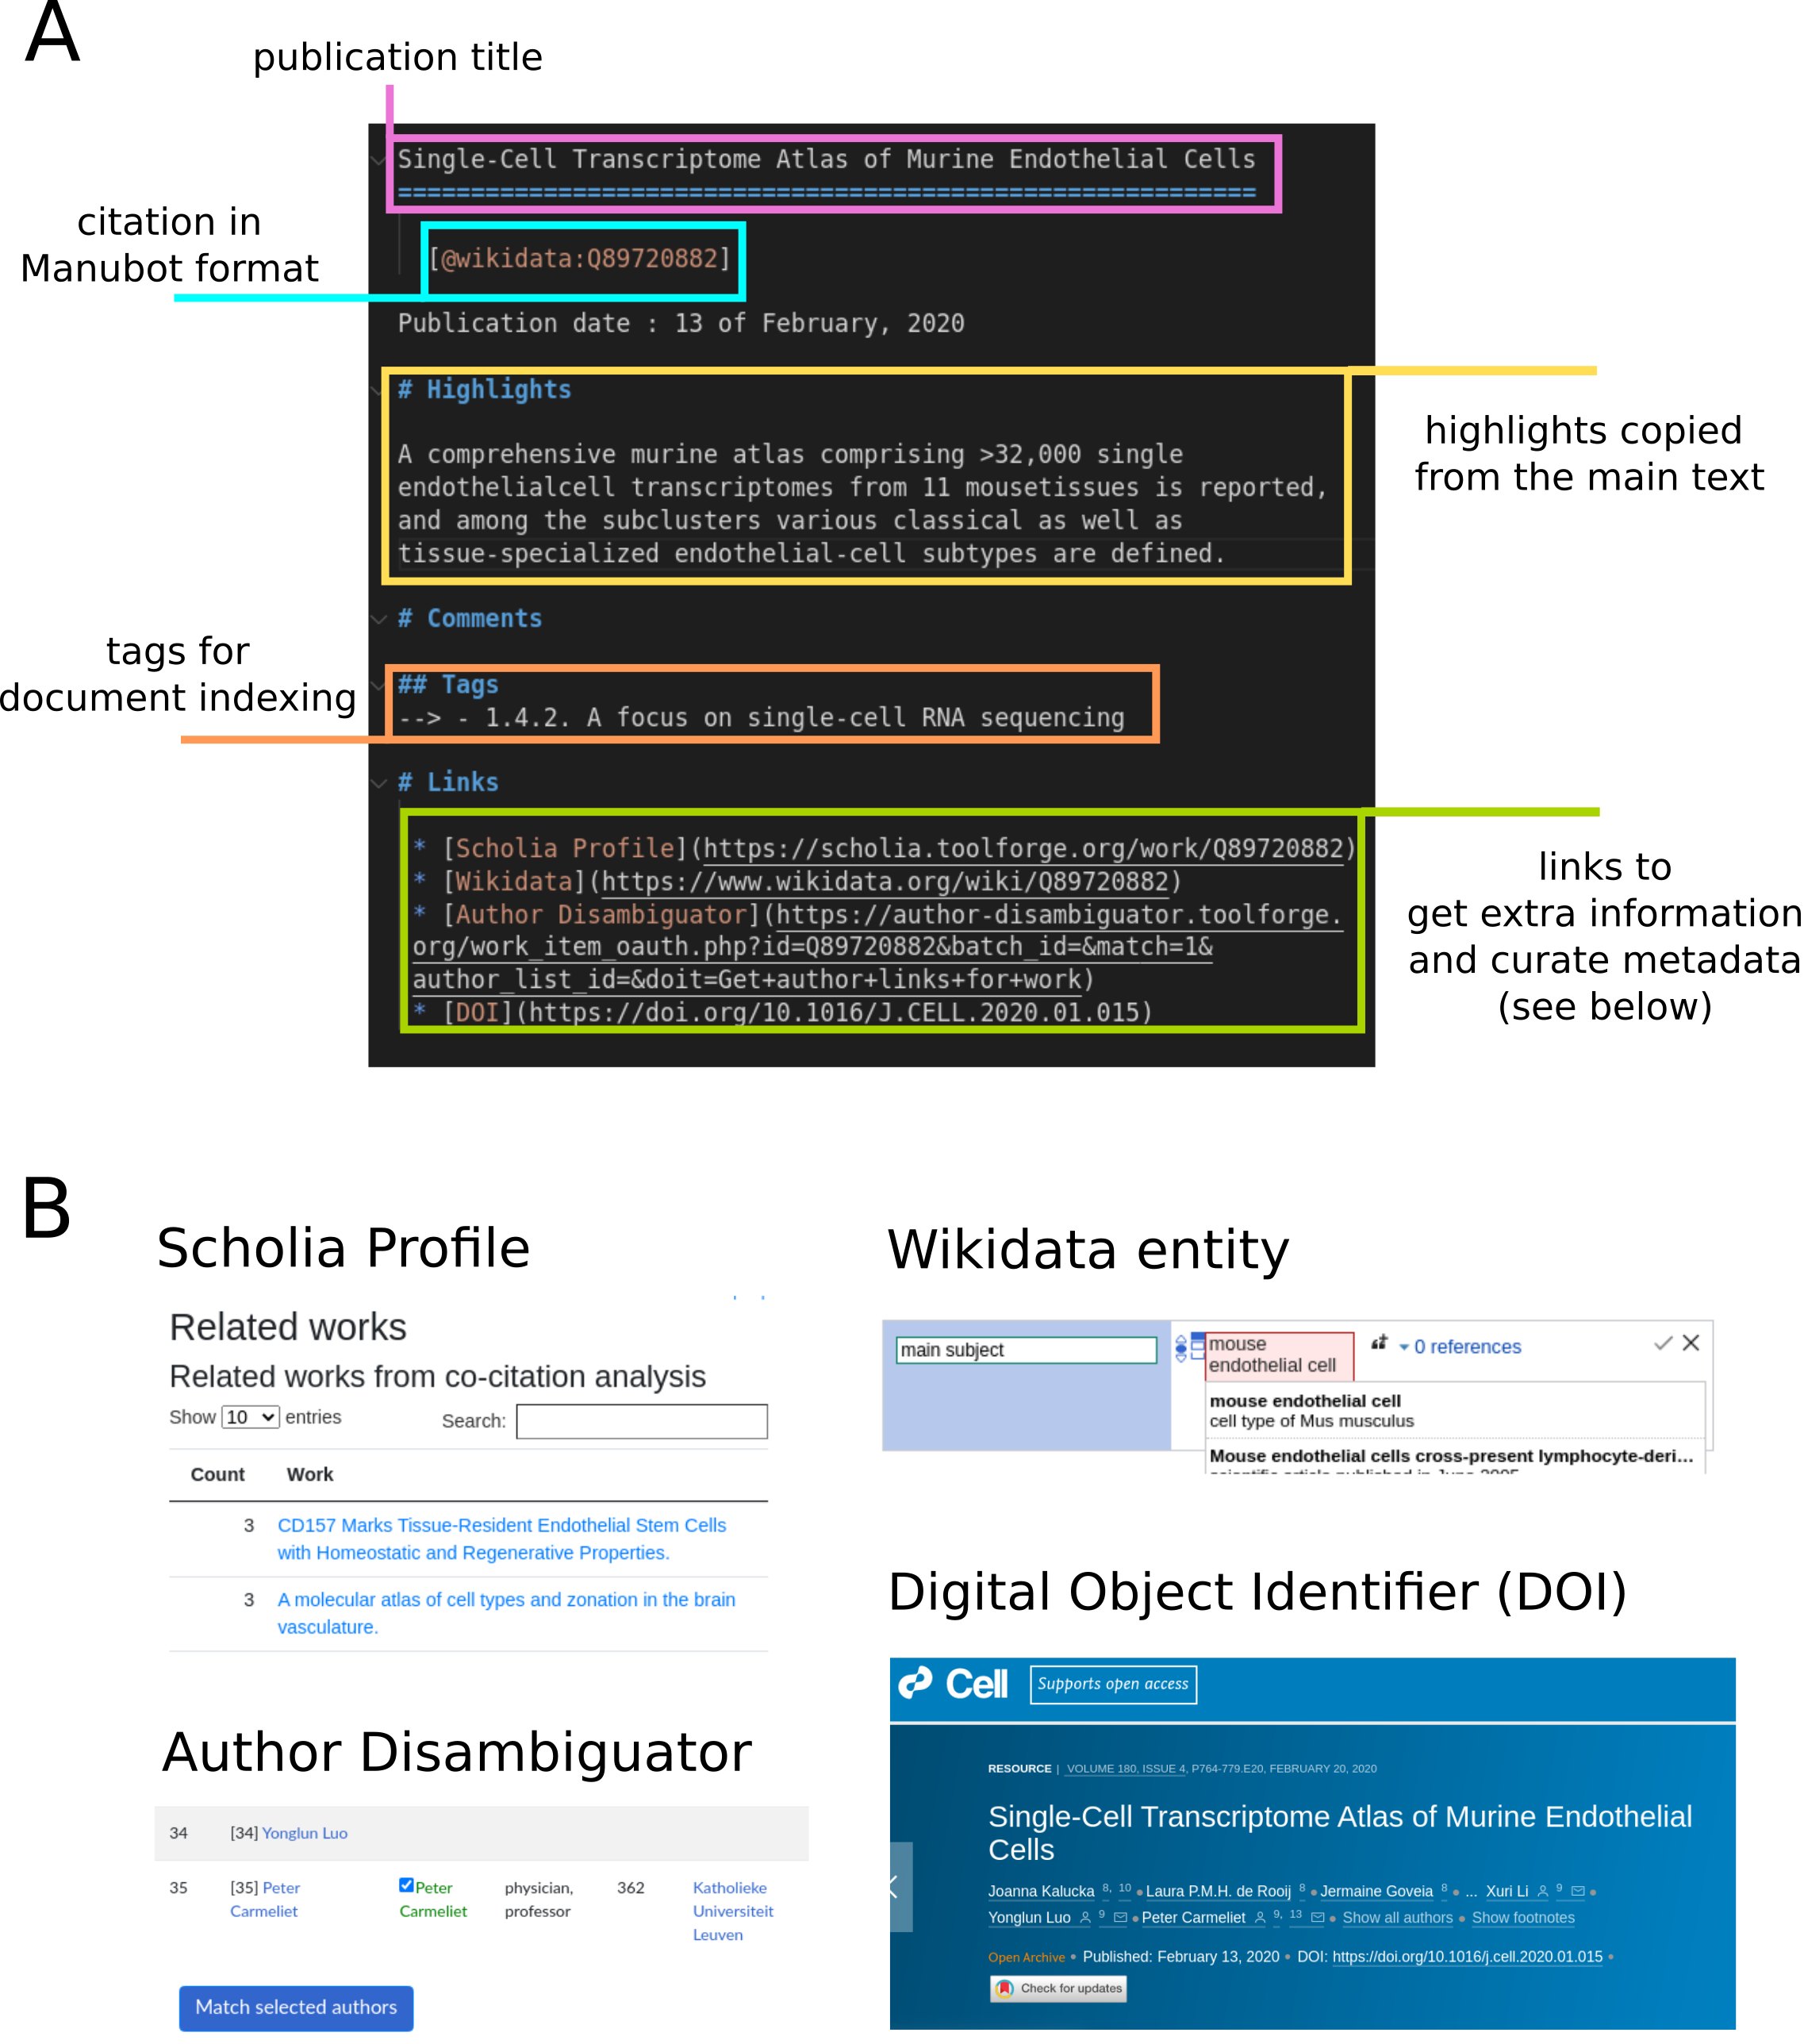
\includegraphics{images/note_taking_station_annotated_with_links.png}
\caption{Wikidata Bib's platform for note taking}\label{fig:notetaking}
}
\end{figure}

The source code for Wikidata Bib is available at https://github.com/lubianat/wikidata\_bib.

\hypertarget{wikidata-bib-as-a-dashboard}{%
\subsection{Wikidata Bib as a dashboard}\label{wikidata-bib-as-a-dashboard}}

The Wikidata Bib system also enables the reader to get statistics on their readings.
Two simple databases are stored on the GitHub repository:
* \texttt{read.ttl} - An RDF document recording the dates in which each article was read.
* \texttt{read.csv} - An simple, human-readable, index connecting QIDs with article titles.
The csv file is only stored for accountability, and as a quick way to glance at the titles read.
The .ttl file, in the other hand, is processed by the \texttt{update\_dashboard.py} script to render 4 different html files under the \texttt{docs/} folder:
- \texttt{index.html}
- \texttt{last\_day.html}
- \texttt{past\_week.html}
- \texttt{past\_month.html}
All files are displayed in a GitHub pages.
In the case of this work, they are displayed at https://lubianat.github.io/wikidata\_bib/.

To organize the code for rendering the dashboard, we created a python package, wbib, and deposited it in PyPi, making it available via \texttt{pip}. {[}\protect\hyperlink{ref-6chnW6cc}{20}/{]}.
The package implements the logic for rendering complex Wikidata-based academic dashboards and is available in GitHub at https://github.com/lubianat/wbib.
It allows the user to build dashboards based on Wikidata records of information such as gender of authors, the region of author\texttt{s\ intitutions,\ topics\ of\ articles\ and\ similar\ metascientific\ information.\ \ The\ dashboard\ is\ composed\ of\ SPARQL\ queries\ written\ for\ the\ Wikidata\ Query\ Service\ {[}@url:https://query.wikidata.org{]}\ \ It\ also\ allows\ users\ to\ feed\ an\ arbitrary\ list\ of\ articles\ and\ obtain\ a\ custom\ dashboard.\ \ Wikidata\ Bib\ obtains\ the\ html\ dashboards\ after\ feeding\ wbib\ the\ lists\ of\ articles\ read\ in\ total\ (}index.html\texttt{)\ or\ in\ pre-determined\ time\ spans\ (}last\_day.html\texttt{,}past\_week.html\texttt{and}past\_month.html` )

\begin{figure}
\hypertarget{fig:dashboard}{%
\centering
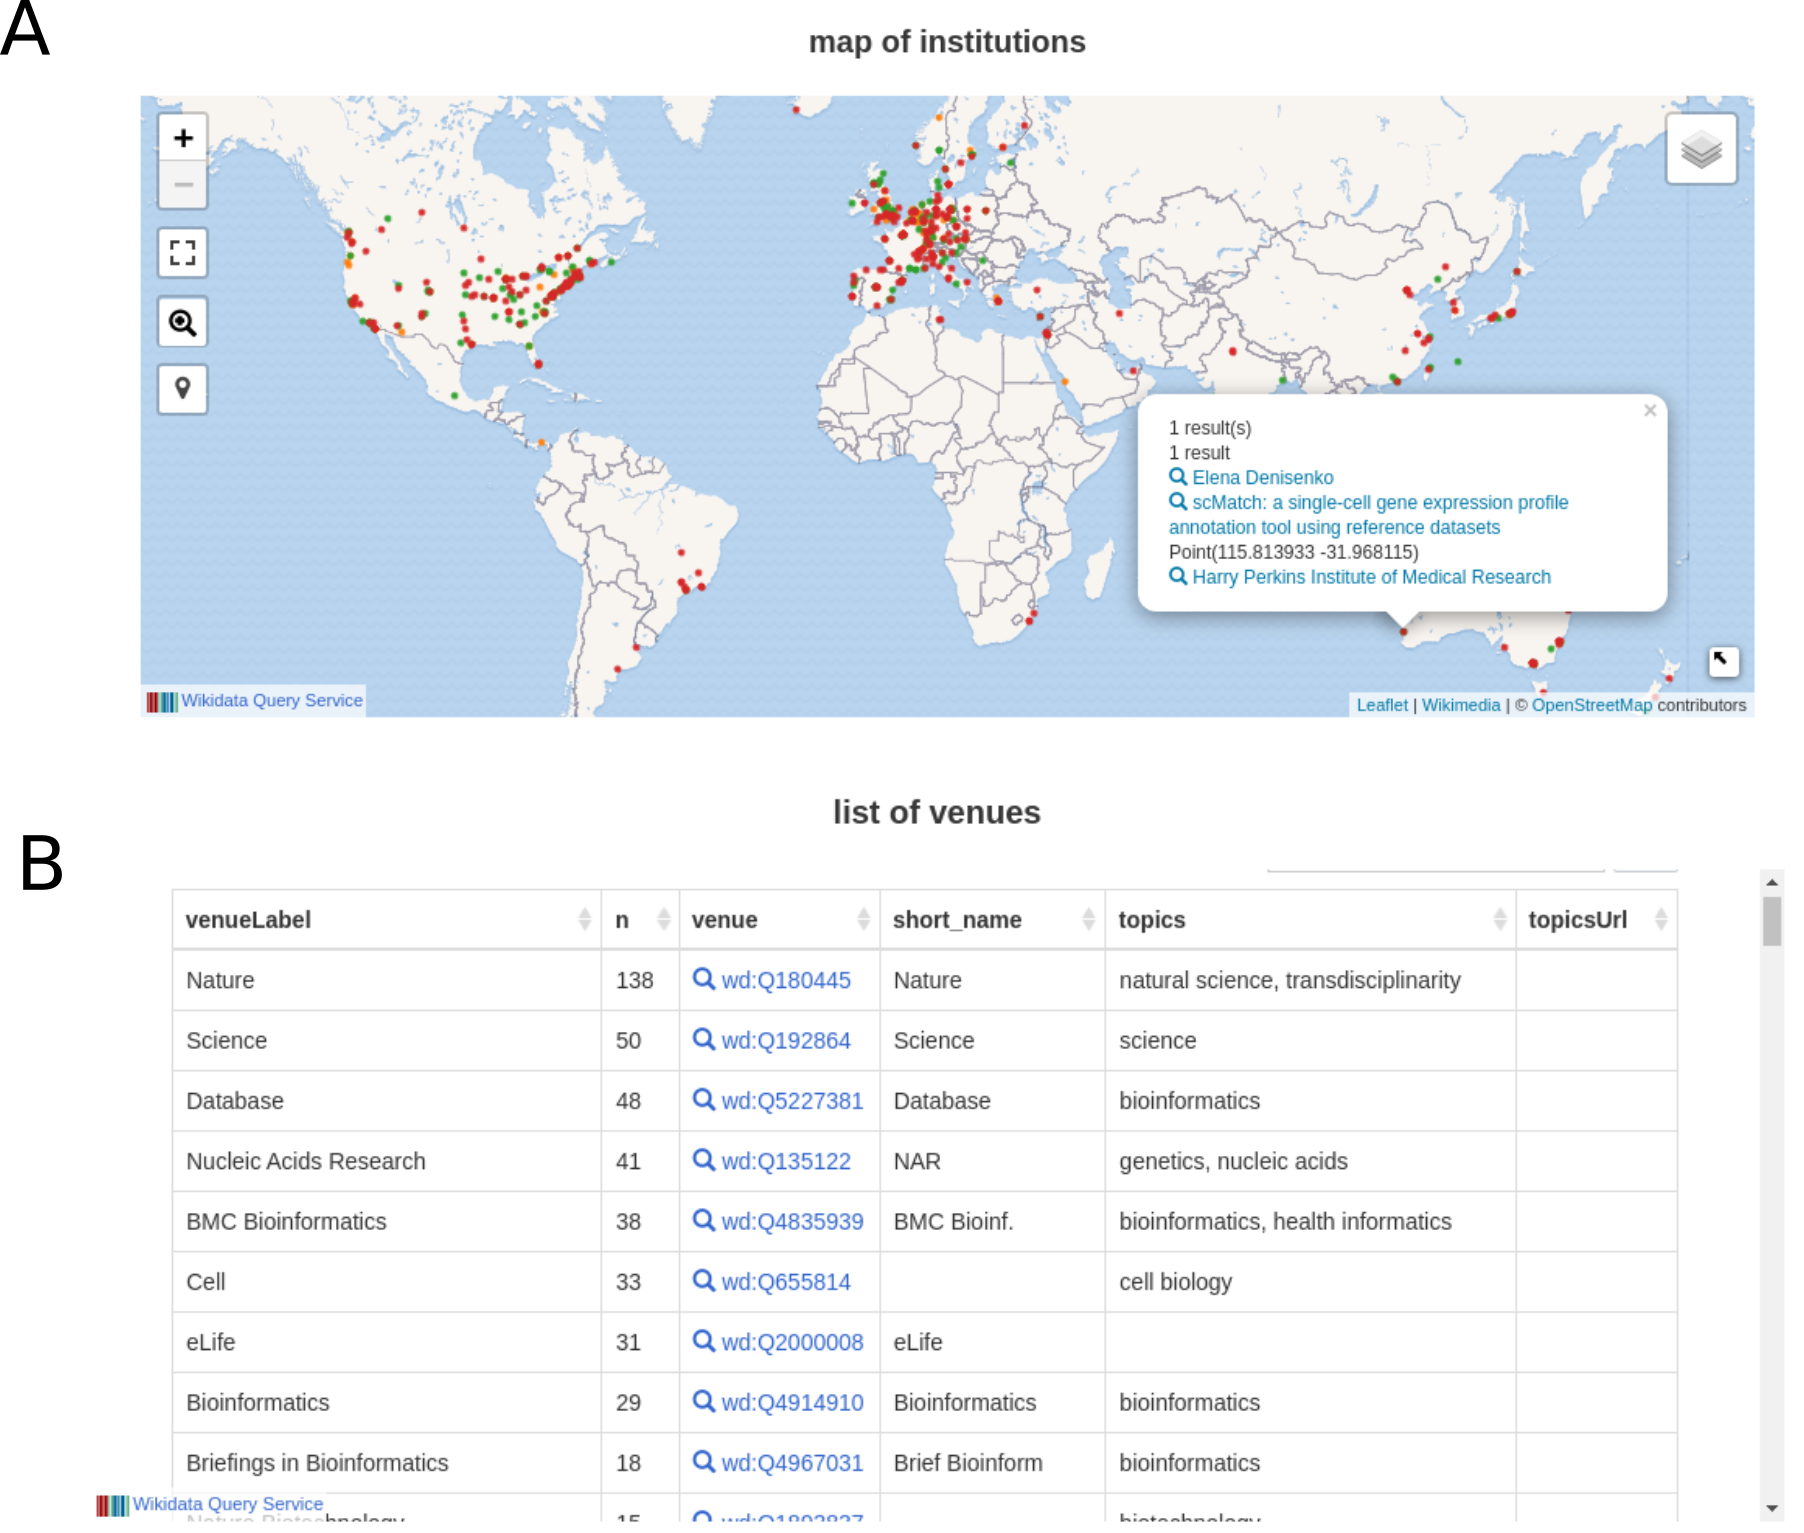
\includegraphics{images/wikidata_bib_display.png}
\caption{Wikidata Bib queries for institutions of authors and most read venues}\label{fig:dashboard}
}
\end{figure}

The dashboard includes not only a basic list of read articles, but also statistics on most read authors and most read venues.
It also displays an interactive map of the instituions of articles read, permitting a glance on geographic biases in activities.
An example of queries is show in \ref{fig:dashboard}.
As the queries are rendered live, they evolve in quality with the growth of Wikidata.
Finally, the clean 5-star-open data format enables users to adapt the queries to include different aspects of Wikidata.
For example, table \ref{tbl:articles_read_hca} showcases 10 articles that (1) I have read in the past year and (2) were authored by a speaker of the 1st Human Cell Atlas Latin America Single Cell RNA-seqData Analysis Workshop {[}\protect\hyperlink{ref-1hag8XE6}{21}/{]}.
One practical application that the dashboard enables, thus, is to identify people in an event, institution or location that the user has read before, therefore catalysing the possibility of colaborations.
Anedoctally, this strategy was tested successfully at Biohackathon Europe 2021 {[}\protect\hyperlink{ref-kHL3NVxk}{22}/{]}, where I used the system both to identify possible collaborators and as a conversation starter.
\textbar workLabel \textbar authors \textbar{}
\textbar-------------------------------------------------------------------------------------------------\textbar--------------------------------------------------------------------------\textbar{}
\textbar A promoter-level mammalian expression atlas \textbar Jay W Shin \textbar{}
\textbar Single-cell RNA-seq reveals new types of human blood dendritic cells, monocytes, and progenitors.\textbar Muzlifah Haniffa \textbar{}
\textbar The Human Cell Atlas. \textbar Musa Mhlanga, Jay W Shin, Muzlifah Haniffa, Menna R Clatworthy, Dana Pe'er\textbar{}
\textbar The Human Cell Atlas: Technical approaches and challenges. \textbar Jay W Shin \textbar{}
\textbar Innate Immune Landscape in Early Lung Adenocarcinoma by Paired Single-Cell Analyses. \textbar Dana Pe'er \textbar{}
\textbar Single cell RNA sequencing of human liver reveals distinct intrahepatic macrophage populations \textbar Sonya A MacParland \textbar{}
\textbar Single-cell reconstruction of the early maternal--fetal interface in humans \textbar Muzlifah Haniffa \textbar{}
\textbar Distinct microbial and immune niches of the human colon \textbar Rasa Elmentaite, Menna R Clatworthy \textbar{}
\textbar A cell atlas of human thymic development defines T cell repertoire formation \textbar Muzlifah Haniffa, Menna R Clatworthy \textbar{}
\textbar Decoding human fetal liver haematopoiesis \textbar Muzlifah Haniffa \textbar{}
Table: Articles read by Tiago Lubiana before 8 December 2021 in which an author was a speaker at HCA Latin America
\{\#tbl:articles\_read\_hca\} \textbar{}

\hypertarget{wikidata-bib-for-curation-of-cells-to-wikidata}{%
\subsection{Wikidata Bib for curation of cells to Wikidata}\label{wikidata-bib-for-curation-of-cells-to-wikidata}}

The Wikidata Bib system was devised originally to allow an overview of the fields of cell classification and biocuration.
However, during the process, it was also repurposed for biocuration of new cell classes in Wikidata.
By fast-tracking the reading of new articles, Wikidata Bib enables an efficient parsing of the literature, and, thus, the identification of previously uncatalogued cell types.

Articles read with Wikidata Bib were screened for the mention of cell types absent from Wikidata.
As discussed on the chapter about the concept of cell type, we considered as a ``cell type'' as as any class of cells described by a domain expert with evidence of reality of its instances.
When a mention of such a class appears in an article, I first verify Wikidata for the existence of a related class.
If it is absent from the platform , I enter a class name, alongside a superclass, and a QID in a Google Spreadsheet, as shown in Figure \ref{fig:biocuration_of_cells}.

The information from the spreadsheet is pulled by a python script, and processed locally with a series of dictionaries that match common terms to Wikidata IDs.
In the example shown in Figure \ref{fig:biocuration_of_cells}, the string ``endothelial cell'' was matched against a manually curated dictionary to the wikidata entry \href{https://www.wikidata.org/wiki/Q11394395}{Q11394395}, the representation of that concept on Wikidata.
After reconciling the data, the script uses the Wikidata Integrator python package {[}\protect\hyperlink{ref-qDI8I4IJ}{23}{]} to insert the new entries on the Wikidata database.
The code for integrating a Google Spreadsheet to Wikidata is available at https://github.com/lubianat/wikidata\_cell\_curation.

\begin{figure}
\hypertarget{fig:biocuration_of_cells}{%
\centering
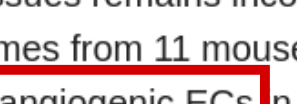
\includegraphics[width=0.85\textwidth,height=\textheight]{images/biocuration_of_cells.png}
\caption{Wikidata Bib was coupled with a biocuration framework for cell types}\label{fig:biocuration_of_cells}
}
\end{figure}

Wikidata contains 2940 subclasses of ``cell (\href{https://www.wikidata.org/wiki/Q7868}{Q7868})'' as of 8 December 2021.
From those, 550 cell classes are specific for humans and 318 are specific for mice.\\
As a comparison, as of 8 of December 2021, Wikidata has more cell classes than the Cell Ontology, which lists 2577 classes.
It is worth noticing that classes on the Cell Ontology are added after careful consideration by ontologists and domain experts, and should be considered of higher quality than the ones on Wikidata.

From the 2940 cell classes on Wikidata, 2812 (95.6\%) have been edited in some way by User:TiagoLubiana, and 1668 (56.7\%) have been created by User:TiagoLubiana.
Edits made to the cells were often connecting a dangling term, created automatically from an Wikipedia page to the cell subclass hierarchy, but also included adding of identifiers, images, markers and other pieces of information.
From the 1668 entities created, approximately 63 species-neutral cell types, 188 human and 188 mouse cell types were added based on PanglaoDB entries (total of 439).
The remaining 1229 entries were created either directly via Wikidata's web interface or using the curation workflow described in this chapter.
Theses statistics are a simple demonstration of how the curation system is efficiently contributing to the status of cell type information on Wikidata.

\begin{figure}
\hypertarget{fig:subclass_of_cell}{%
\centering
\includegraphics[width=0.85\textwidth,height=\textheight]{https://keep.google.com/u/0/media/v2/1WoYkTz0M-ew_Tay-DpmOr2zyyCalnmsyd_2Ysq3pyNaJ7R5CIQnfdvZTDviBcvc/18W-amXz1489obuE7Tqb-AQHZKa-x-aVaH7QsO3x7Cy7lz-4a6AMzaGdLffzB?sz=512\&accept=image\%2Fgif\%2Cimage\%2Fjpeg\%2Cimage\%2Fjpg\%2Cimage\%2Fpng\%2Cimage\%2Fwebp}
\caption{Subclasses of ``cell'' on Wikidata}\label{fig:subclass_of_cell}
}
\end{figure}

\hypertarget{wikidata-and-the-cell-ontology-interplay}{%
\subsection{Wikidata and the Cell Ontology interplay}\label{wikidata-and-the-cell-ontology-interplay}}

The contributions to cell types on Wikidata will be of most value if they are integrated to the current state-of-art of knowledge representation.
Arguably, the Cell Ontology is the current leading source of cell type identifiers in the context of the Human Cell Atlas project.{[}\protect\hyperlink{ref-qT8WxqjA}{24}{]}
Thus, it is crucial that data about cell types on Wikidata is connected to the Cell Ontology.

To start the improvement in the interplay of both databases, we proposed and got approval of a specific Wikidata identifier for the Cell Ontology, the ``Cell Ontology ID'' (\url{https://www.wikidata.org/wiki/Property:P7963}).
IDs can be added to Wikidata entities and connect them to external databases enabling integrative SPARQL queries.
Besides using the common Wikidata interface, one can crowd-curate identifiers via 3rd-party service, Mix'N'Match, which provides an user-friendly framework for connecting idenfier catalogs to Wikidata. {[}\protect\hyperlink{ref-JgiKEEdq}{25}/?p=114{]}, as seen in Figure \ref{fig:mixn_match_cl}.
Logically, we created a Mix'N'Match catalog for harmonizing Cell Ontology IDs to Wikidata (\url{https://mix-n-match.toolforge.org/\#/catalog/4719}), harnessing the community support for the task.

\begin{figure}
\hypertarget{fig:mixnmatch_cl}{%
\centering
\includegraphics[width=0.85\textwidth,height=\textheight]{https://pointstodots.files.wordpress.com/2021/09/image-17.png}
\caption{Mix'N'Match curation system}\label{fig:mixnmatch_cl}
}
\end{figure}

As of early December 2021, more than 700 Cell Ontology IDs have been manually matched to Wikidata.
The integration already enables queries that harness the previously existing information on Wikidata for Cell Ontology - based applications.
For example, one can query Wikidata items that have (1) a crossref to a CL ID (2) a picture in Wikimedia Commons (\url{https://w.wiki/4F6e}, Figure \ref{fig:cl_images}).
The different possibilities of mutual benefit between the Cell Ontology and Wikidata will continue to be explored in the next years of this PhD project.

\includegraphics{https://user-images.githubusercontent.com/7917951/137942026-7645f368-d62a-4434-be05-083555cf0757.png} \{\#fig:cl\_images width=``85\%''\}

\hypertarget{final-considerations-and-next-steps}{%
\section{Final considerations and next steps}\label{final-considerations-and-next-steps}}

To sum up, this PhD research project aims at improving knowledge representation in the context of the Human Cell Atlas.
It is composed by a mixture of theoretical studies on conceptual modelling, practical contributions to knowledge organization projects, (mainly the Cell Ontology and Wikidata), explorations of the data to generate biomedical insights and the development of a technical framework for organized reading.
By approaching the object of study from a new perspective, we hope not only to make sizeable contributions, but to promote discussion and fruitful conflation of approaches.

The next years of study will be devoted to improving the projects presented here into mature, useful objects.
We hope to improve the interplay of Wikidata and Cell Ontology, developing frameworks to combine community- and expert- based curation of knowledge on cell types.
Furthermore, we plan to integrate Wikidata to current single-cell RNA-sequencing pipelines by adapting ontology-based R packages (as OnClass {[}\protect\hyperlink{ref-sW6aNZJB}{26}{]} and ontoProc{[}\protect\hyperlink{ref-15YmDXALp}{27}{]})) to use Wikidata.
Finally, we aim at moving the Wikidata Bib system to a well documented, user-friendly mature system, testing usability with other academics and distributing it as a durable open-source project.

\hypertarget{additional-work}{%
\section{Additional Work}\label{additional-work}}

\hypertarget{collaborations-and-manuscripts}{%
\subsection{Collaborations and manuscripts}\label{collaborations-and-manuscripts}}

\hypertarget{fcoex}{%
\subsubsection{fcoex}\label{fcoex}}

During the initial course of this PhD work, we also completed the development and reportin of \emph{fcoex}, an R package for investigating cellular phenotypes using co-expression networks. {[}\protect\hyperlink{ref-MxIeSJYt}{28}{]} The software was mantained to withstand new releases of dependencies and new R version, and \emph{WAS PUBLISHED AS A PRE\_PRINT ADD HERE THE LINK}.

\hypertarget{wikidata-bots}{%
\subsubsection{Wikidata Bots}\label{wikidata-bots}}

Alongside the editing of cell-type information on Wikidata, I have joined different efforts to improve biological information on Wikidata.
I have collaborated with the ComplexPortal curators, as part of the Virtual Elixir BioHackathon 2020 (https://github.com/virtual-biohackathons/covid-19-bh20/wiki) and for the following year, to build an Wikidata Bot to integrate information on protein complexes to Wikidata. An overview of the Wikidata integration is in Figure \ref{fig:complexportal}, presented in an article published in Nucleic Acid Research (re-use of the image and legend possible under the CC-BY license of the article). {[}\protect\hyperlink{ref-CQRJ53gu}{29}{]}
\includegraphics{https://oup.silverchair-cdn.com/oup/backfile/Content_public/Journal/nar/PAP/10.1093_nar_gkab991/2/gkab991fig3.jpeg?Expires=1641821957\&Signature=RK-es18S~Qh6vGQE~61i6u4prMuij8kVTbrjN6WUJLfYHOAhUhx9qQorBxROohjLLxbHvZ2YK9e7EwlI9HjVeNoGZ2PJs0Pv78Y31MdZLY8FeLYI2E4azwrqRyv9q0AH8QL3RorWZV1AhOb9bl-44Mr97Q~9MWzeTDnQQbxpCnGLG~YoG49kocD5KE~dmTSQdkXBU7kZnuGM1NPqMHo5ZDUoCRFwmTbLvd4kXoH~6CTyqx4ruQRIO-ks4Q0FUjYnxGX18gCFvoO2LMPZUPrQjTgD35RrVAkLs91Ur6BQHUuZ-ZsE3Iag3mBDu27vT9Jr93bOj0i9wz~surTtEGATgw__\&Key-Pair-Id=APKAIE5G5CRDK6RD3PGA}

I have also collaborated with the Cellosaurus database {[}\protect\hyperlink{ref-1DguATd9G}{30}{]} to revive the CellosaurusBot {[}\protect\hyperlink{ref-lMQxhx3q}{31}{]}, responsible for updating the metadata on more than 100,000 cell lines on Wikidata. The bot code, written in Python, was completely refactored, and is run by me semi-automatically after the Cellosaurus database releases. A write-up of he integration is in progress, and is planned for release/submisson in the first semester of 2022.

\hypertarget{systematic-reviews-and-publishing-of-intermediary-tables}{%
\subsubsection{Systematic Reviews and publishing of intermediary tables}\label{systematic-reviews-and-publishing-of-intermediary-tables}}

Finally, in a collaboration with Olavo Amaral and Kleber, from the Brazilian Reproducibility Initiative {[}\protect\hyperlink{ref-F2mYjDJ0}{32}{]} I wrote a commentary on the value of publishing intermediate datasets as citable products. {[}\protect\hyperlink{ref-HbZ13t8l}{33}/{]}
The pieces discuss the value of small curations done both in systematic reviews and by experimentalists in the course of their research projects. Published curation tables can serve as a source for improving the ecosystem of open knowledge, not less by reconciliation to Wikidata (thereby bridging the commentary with this project)

\hypertarget{wisecube---enterprise-biomedical-question-and-answering}{%
\subsubsection{WiseCube - enterprise biomedical question and answering}\label{wisecube---enterprise-biomedical-question-and-answering}}

During a part of this project, I have worked part-time as a consultant for the Wisecube company, based in Seattle, United States. {[}\protect\hyperlink{ref-gdYsBE7d}{34}/{]}
The job was approved by FAPESP, and consisted mainly in writing SPARQL queries that probe Wikidata for answers to the questions posed by the BioASQ competition. {[}\protect\hyperlink{ref-rkXotO9x}{35}{]}
It also entails on-demand curation of biomedical topics on Wikidata based on requests by pharmaceutical companies as well as the development of dashboards targeted at providing insights to customers.

\hypertarget{awards-and-participation-in-events}{%
\subsection{Awards and participation in events}\label{awards-and-participation-in-events}}

During the initial course of this PhD project, I have participated in several events:

\begin{itemize}
\tightlist
\item
  (Feb-2021) Presented an open talk at the ``Semana da Bioinformática'' event about modelling of biological systems (1020 views as of December 2021) {[}\protect\hyperlink{ref-1C9uHr1Zk}{36}, =VDvCxskIGEI{]}
\item
  (Jun-Aug 2021) Helped to organize the No-Budget-Science HackWeek virtual hackathon {[}\protect\hyperlink{ref-12LOzmXRs}{37}{]}
\item
  (Jul - 2021) Presented the work ``Wikidata for 5-star Linked Open Databases: A case study of PanglaoDB'' at the Bio-Ontologies section of the Annual International Conference on Intelligent Systems for Molecular Biology. {[}\protect\hyperlink{ref-SALI6Ywb}{38}{]}. The presentation was awarded the best
\item
  (Jul - 2021) Awarded the 2nd place in the International Society for Computational Biology (ISCB) Wikipedia Competition for the contributions to the Wikipedia page on Biocuration (\url{https://en.wikipedia.org/wiki/Biocuration}) {[}\protect\hyperlink{ref-IJG65hFm}{39}{]}
\item
  (Nov - 2021) Managed a project during BioHackathon Europe 2021, in Barcelona, Spain, on the representation of ELIXIR information on Wikidata. {[}\protect\hyperlink{ref-14Wi842eZ}{40}{]}
\end{itemize}

\hypertarget{course-work}{%
\subsection{Course work}\label{course-work}}

During the first year of the PhD program, I took 4 different classes, acquiring a total of 36 academic credits.
Figure \ref{fig:courses_taken} displays the disciplines taken, available only in portuguese.

\begin{figure}
\hypertarget{fig:courses_taken}{%
\centering
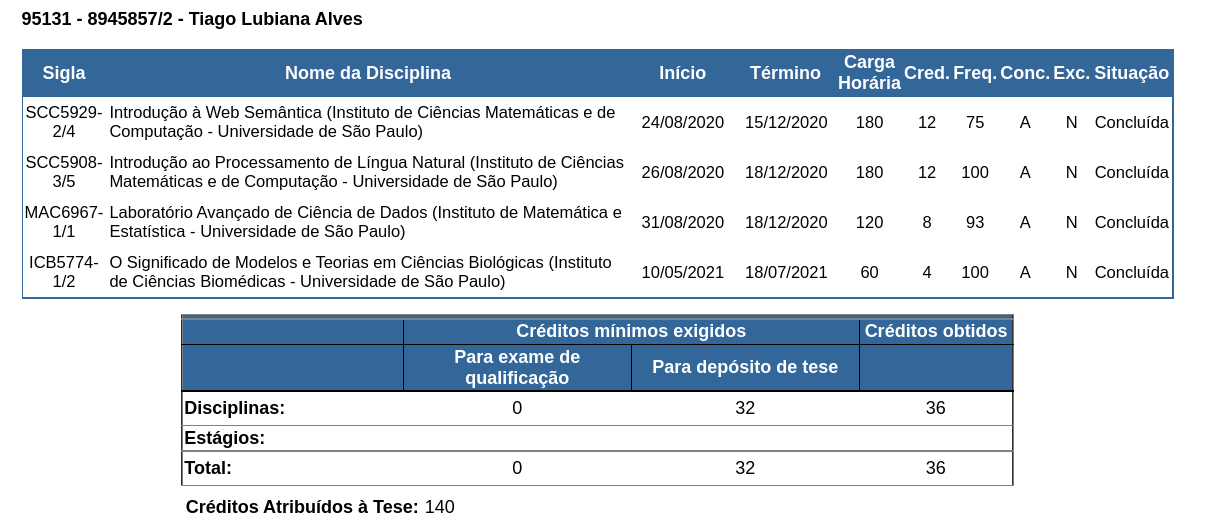
\includegraphics{images/janus_courses_taken.png}
\caption{Courses taken}\label{fig:courses_taken}
}
\end{figure}

\hypertarget{references}{%
\subsection{References}\label{references}}

\hypertarget{refs}{}
\begin{CSLReferences}{0}{0}
\leavevmode\vadjust pre{\hypertarget{ref-pNGap1Du}{}}%
\CSLLeftMargin{1. }
\CSLRightInline{\textbf{An era of single-cell genomics consortia}
\CSLBlock{Yoshinari Ando, Andrew T Kwon, Jay W Shin} \emph{Experimental and Molecular Medicine} (2020-09-15) \url{https://www.wikidata.org/wiki/Q99418649}
\CSLBlock{DOI: \href{https://doi.org/10.1038/s12276-020-0409-x}{10.1038/s12276-020-0409-x}}}

\leavevmode\vadjust pre{\hypertarget{ref-1GmbExweg}{}}%
\CSLLeftMargin{2. }
\CSLRightInline{\textbf{The Human Cell Atlas.}
\CSLBlock{Aviv Regev, Sarah Teichmann, Eric Lander, Amir Giladi, Christophe Benoist, Ewan Birney, Bernd Bodenmiller, Peter Campbell, Piero Carninci, Menna R Clatworthy, \ldots{} Human Cell Atlas Meeting Participants} \emph{eLife} (2017-12-05) \url{https://www.wikidata.org/wiki/Q46368626}
\CSLBlock{DOI: \href{https://doi.org/10.7554/elife.27041}{10.7554/elife.27041}}}

\leavevmode\vadjust pre{\hypertarget{ref-tjdjR2Xf}{}}%
\CSLLeftMargin{3. }
\CSLRightInline{\textbf{The Human Cell Atlas and equity: lessons learned}
\CSLBlock{Partha P Majumder, Musa M Mhlanga, Alex K Shalek} \emph{Nature Medicine} (2020-10-01) \url{https://www.wikidata.org/wiki/Q100491106}
\CSLBlock{DOI: \href{https://doi.org/10.1038/s41591-020-1100-4}{10.1038/s41591-020-1100-4}}}

\leavevmode\vadjust pre{\hypertarget{ref-kkwRTArg}{}}%
\CSLLeftMargin{4. }
\CSLRightInline{\textbf{The Human Cell Atlas White Paper}
\CSLBlock{Aviv Regev, Sarah Teichmann, Orit Rozenblatt-Rosen, Michael JT Stubbington, Kristin Ardlie, Amir Giladi, Paola Arlotta, Gary D Bader, Christophe Benoist, Moshe Biton, \ldots{} Human Cell Atlas Organizing Committee} (2018-10-11) \url{https://www.wikidata.org/wiki/Q104450645}}

\leavevmode\vadjust pre{\hypertarget{ref-1DSEIjFha}{}}%
\CSLLeftMargin{5. }
\CSLRightInline{\textbf{Everyone needs a data-management plan}
\CSLBlock{Nature} (2018-03-15) \url{https://www.wikidata.org/wiki/Q56524391}
\CSLBlock{DOI: \href{https://doi.org/10.1038/d41586-018-03065-z}{10.1038/d41586-018-03065-z}}}

\leavevmode\vadjust pre{\hypertarget{ref-zDRzmIGu}{}}%
\CSLLeftMargin{6. }
\CSLRightInline{\textbf{About the Data Coordination Platform}
\CSLBlock{HCA Data Portal} \url{https://data.humancellatlas.org/about/}}

\leavevmode\vadjust pre{\hypertarget{ref-kX6KnbUo}{}}%
\CSLLeftMargin{7. }
\CSLRightInline{\textbf{Mapping the Human Body at the Cellular Level}
\CSLBlock{HCA Data Portal} \url{https://data.humancellatlas.org/}}

\leavevmode\vadjust pre{\hypertarget{ref-chGii6yw}{}}%
\CSLLeftMargin{8. }
\CSLRightInline{\textbf{CellMarker: a manually curated resource of cell markers in human and mouse}
\CSLBlock{Xinxin Zhang, Yujia Lan, Jinyuan Xu, Fei Quan, Erjie Zhao, Chunyu Deng, Tao Luo, Liwen Xu, Gaoming Liao, Min Yan, \ldots{} Yun Xiao} \emph{Nucleic Acids Research} (2019-01-01) \url{https://www.wikidata.org/wiki/Q56984510}
\CSLBlock{DOI: \href{https://doi.org/10.1093/nar/gky900}{10.1093/nar/gky900}}}

\leavevmode\vadjust pre{\hypertarget{ref-rhRRCtlA}{}}%
\CSLLeftMargin{9. }
\CSLRightInline{\textbf{Cell Markers}
\CSLBlock{Konstantin Yakimchuk} \emph{Materials and Methods} (2013-05-02) \url{https://doi.org/ghq494}
\CSLBlock{DOI: \href{https://doi.org/10.13070/mm.en.3.183}{10.13070/mm.en.3.183}}}

\leavevmode\vadjust pre{\hypertarget{ref-4AEy2xhQ}{}}%
\CSLLeftMargin{10. }
\CSLRightInline{\textbf{CellFinder: a cell data repository}
\CSLBlock{Harald Stachelscheid, Stefanie Seltmann, Fritz Lekschas, Jean-Fred Fontaine, Nancy Mah, Mariana Lara Neves, Miguel A Andrade-Navarro, Ulf Leser, Andreas Kurtz} \emph{Nucleic Acids Research} (2013-12-03) \url{https://www.wikidata.org/wiki/Q28660708}
\CSLBlock{DOI: \href{https://doi.org/10.1093/nar/gkt1264}{10.1093/nar/gkt1264}}}

\leavevmode\vadjust pre{\hypertarget{ref-6uWWsiSq}{}}%
\CSLLeftMargin{11. }
\CSLRightInline{\textbf{SHOGoiN: Shogoin Human Omics database for the Generation of iPS and Normal cells} \url{https://stemcellinformatics.org/}}

\leavevmode\vadjust pre{\hypertarget{ref-uYuz0opI}{}}%
\CSLLeftMargin{12. }
\CSLRightInline{\textbf{Wikipedia, the free encyclopedia} \url{https://en.wikipedia.org/wiki/Main_Page}}

\leavevmode\vadjust pre{\hypertarget{ref-rPKBwmYh}{}}%
\CSLLeftMargin{13. }
\CSLRightInline{\textbf{Como fazer um fichamento}
\CSLBlock{Priscilla de Carvalho Nunes disse} \emph{Blog da Biblioteca da ECA-USP} (2019-09-30) \url{https://bibliotecadaeca.wordpress.com/2019/09/30/como-fazer-um-fichamento/}}

\leavevmode\vadjust pre{\hypertarget{ref-PKhuVRW8}{}}%
\CSLLeftMargin{14. }
\CSLRightInline{\url{https://www.youtube.com/playlist?list}}

\leavevmode\vadjust pre{\hypertarget{ref-1HBVPtZGp}{}}%
\CSLLeftMargin{15. }
\CSLRightInline{\textbf{Come si fa una tesi di laurea} \url{https://www.wikidata.org/wiki/Q3684178}}

\leavevmode\vadjust pre{\hypertarget{ref-15luL9zZC}{}}%
\CSLLeftMargin{16. }
\CSLRightInline{\textbf{Unpaywall} \url{https://unpaywall.org/}}

\leavevmode\vadjust pre{\hypertarget{ref-13HqB23xH}{}}%
\CSLLeftMargin{17. }
\CSLRightInline{\textbf{Clean Code: A Handbook of Agile Software Craftsmanship} \url{https://www.wikidata.org/wiki/Q109996684}}

\leavevmode\vadjust pre{\hypertarget{ref-hxzL9pmm}{}}%
\CSLLeftMargin{18. }
\CSLRightInline{\textbf{Scholia, Scientometrics and Wikidata}
\CSLBlock{Finn Årup Nielsen, Daniel Mietchen, Egon Willighagen} \emph{The Semantic Web: ESWC 2017 Satellite Events} (2017-10-01) \url{https://www.wikidata.org/wiki/Q41799194}
\CSLBlock{DOI: \href{https://doi.org/10.1007/978-3-319-70407-4_36}{10.1007/978-3-319-70407-4\_36}}}

\leavevmode\vadjust pre{\hypertarget{ref-1A9RvszKC}{}}%
\CSLLeftMargin{19. }
\CSLRightInline{\textbf{Wikidata:Tools/Author Disambiguator - Wikidata} \url{https://www.wikidata.org/wiki/Wikidata:Tools/Author_Disambiguator}}

\leavevmode\vadjust pre{\hypertarget{ref-6chnW6cc}{}}%
\CSLLeftMargin{20. }
\CSLRightInline{\textbf{wbib: A helper for building Wikidata-based literature dashboards via SPARQL queries.}
\CSLBlock{Tiago Lubiana} \url{https://github.com/lubianat/wbib}}

\leavevmode\vadjust pre{\hypertarget{ref-1hag8XE6}{}}%
\CSLLeftMargin{21. }
\CSLRightInline{\textbf{HCA Latin America - 2021 Workshop} \url{https://www.humancellatlas.org/hca-latin-america-2021-workshop/}}

\leavevmode\vadjust pre{\hypertarget{ref-kHL3NVxk}{}}%
\CSLLeftMargin{22. }
\CSLRightInline{\textbf{BioHackathon Europe} \url{https://biohackathon-europe.org/}}

\leavevmode\vadjust pre{\hypertarget{ref-qDI8I4IJ}{}}%
\CSLLeftMargin{23. }
\CSLRightInline{\textbf{GitHub - SuLab/WikidataIntegrator: A Wikidata Python module integrating the MediaWiki API and the Wikidata SPARQL endpoint}
\CSLBlock{GitHub} \url{https://github.com/SuLab/WikidataIntegrator}}

\leavevmode\vadjust pre{\hypertarget{ref-qT8WxqjA}{}}%
\CSLLeftMargin{24. }
\CSLRightInline{\textbf{Cell type ontologies of the Human Cell Atlas}
\CSLBlock{David Osumi-Sutherland, Chuan Xu, Maria Keays, Adam P Levine, Peter V Kharchenko, Aviv Regev, Ed Lein, Sarah Teichmann} \emph{Nature Cell Biology} (2021-11-01) \url{https://www.wikidata.org/wiki/Q109755180}
\CSLBlock{DOI: \href{https://doi.org/10.1038/s41556-021-00787-7}{10.1038/s41556-021-00787-7}}}

\leavevmode\vadjust pre{\hypertarget{ref-JgiKEEdq}{}}%
\CSLLeftMargin{25. }
\CSLRightInline{\textbf{The Whelming › Tech, tools, and tribulations}
\CSLBlock{Scott Allan Wallick} \url{http://magnusmanske.de/wordpress/}}

\leavevmode\vadjust pre{\hypertarget{ref-sW6aNZJB}{}}%
\CSLLeftMargin{26. }
\CSLRightInline{\textbf{Leveraging the Cell Ontology to classify unseen cell types}
\CSLBlock{Sheng Wang, Angela Oliveira Pisco, Aaron McGeever, Maria Brbić, Marinka Žitnik, Spyros Darmanis, Jure Leskovec, Jim Karkanias, Russ Altman} \emph{Nature Communications} (2021-09-21) \url{https://www.wikidata.org/wiki/Q108929315}
\CSLBlock{DOI: \href{https://doi.org/10.1038/s41467-021-25725-x}{10.1038/s41467-021-25725-x}}}

\leavevmode\vadjust pre{\hypertarget{ref-15YmDXALp}{}}%
\CSLLeftMargin{27. }
\CSLRightInline{\textbf{ontoProc: processing of ontologies of anatomy, cell lines, and so on} \url{https://www.wikidata.org/wiki/Q101074371}}

\leavevmode\vadjust pre{\hypertarget{ref-MxIeSJYt}{}}%
\CSLLeftMargin{28. }
\CSLRightInline{\textbf{fcoex: FCBF-based Co-Expression Networks for Single Cells}
\CSLBlock{Tiago Lubiana, Helder Nakaya} \emph{Bioconductor version: Release (3.14)} (2021) \url{https://bioconductor.org/packages/fcoex/}}

\leavevmode\vadjust pre{\hypertarget{ref-CQRJ53gu}{}}%
\CSLLeftMargin{29. }
\CSLRightInline{\textbf{Complex Portal 2022: new curation frontiers}
\CSLBlock{Birgit HM Meldal, Livia Perfetto, Colin Combe, Tiago Lubiana, João Vitor Ferreira~Cavalcante, Hema Bye-A-Jee, Andra Waagmeester, Noemi del-Toro, Anjali Shrivastava, Elisabeth Barrera, \ldots{} Sandra Orchard} \emph{Nucleic Acids Research} (2021-10-29) \url{https://www.wikidata.org/wiki/Q109348309}
\CSLBlock{DOI: \href{https://doi.org/10.1093/nar/gkab991}{10.1093/nar/gkab991}}}

\leavevmode\vadjust pre{\hypertarget{ref-1DguATd9G}{}}%
\CSLLeftMargin{30. }
\CSLRightInline{\textbf{The Cellosaurus, a cell-line knowledge resource.}
\CSLBlock{Amos Bairoch} \emph{Journal of Biomolecular Techniques} (2018-05-01) \url{https://www.wikidata.org/wiki/Q54370168}
\CSLBlock{DOI: \href{https://doi.org/10.7171/jbt.18-2902-002}{10.7171/jbt.18-2902-002}}}

\leavevmode\vadjust pre{\hypertarget{ref-lMQxhx3q}{}}%
\CSLLeftMargin{31. }
\CSLRightInline{\textbf{User:CellosaurusBot - Wikidata} \url{https://www.wikidata.org/wiki/User:CellosaurusBot}}

\leavevmode\vadjust pre{\hypertarget{ref-F2mYjDJ0}{}}%
\CSLLeftMargin{32. }
\CSLRightInline{\textbf{The Brazilian Reproducibility Initiative}
\CSLBlock{Ana P Wasilewska-Sampaio, Olavo Bohrer Amaral, Kleber Neves, Ana P Wasilewska-Sampaio, Clarissa FD Carneiro, Olavo Bohrer Amaral, Clarissa FD Carneiro} \emph{eLife} (2019-02-05) \url{https://www.wikidata.org/wiki/Q61799268}
\CSLBlock{DOI: \href{https://doi.org/10.7554/elife.41602}{10.7554/elife.41602}}}

\leavevmode\vadjust pre{\hypertarget{ref-HbZ13t8l}{}}%
\CSLLeftMargin{33. }
\CSLRightInline{\url{https://osf.io/preprints/metaarxiv/vbwa9}}

\leavevmode\vadjust pre{\hypertarget{ref-gdYsBE7d}{}}%
\CSLLeftMargin{34. }
\CSLRightInline{\textbf{Wisecube AI \textbar{} Knowledge Graph Engine} \url{https://www.wisecube.ai/}}

\leavevmode\vadjust pre{\hypertarget{ref-rkXotO9x}{}}%
\CSLLeftMargin{35. }
\CSLRightInline{\textbf{An overview of the BIOASQ large-scale biomedical semantic indexing and question answering competition}
\CSLBlock{George Tsatsaronis, Georgios Balikas, Prodromos Malakasiotis, Ioannis Partalas, Matthias Zschunke, Michael R Alvers, Dirk Weissenborn, Anastasia Krithara, Sergios Petridis, Dimitris Polychronopoulos, \ldots{} Georgios Paliouras} \emph{BMC Bioinformatics} (2015-04-30) \url{https://www.wikidata.org/wiki/Q28646342}
\CSLBlock{DOI: \href{https://doi.org/10.1186/s12859-015-0564-6}{10.1186/s12859-015-0564-6}}}

\leavevmode\vadjust pre{\hypertarget{ref-1C9uHr1Zk}{}}%
\CSLLeftMargin{36. }
\CSLRightInline{\textbf{YouTube} \url{https://www.youtube.com/}}

\leavevmode\vadjust pre{\hypertarget{ref-12LOzmXRs}{}}%
\CSLLeftMargin{37. }
\CSLRightInline{\textbf{No Budget Science Hack Week}
\CSLBlock{reprodutibilidade} \url{https://www.reprodutibilidade.bio.br/hack-week-2021}}

\leavevmode\vadjust pre{\hypertarget{ref-SALI6Ywb}{}}%
\CSLLeftMargin{38. }
\CSLRightInline{\textbf{Wikidata for 5-star Linked Open Databases: A case study of PanglaoDB}
\CSLBlock{Tiago Lubiana, João Vitor Ferreira Cavalcante} \emph{Zenodo} (2021-12-01) \url{https://doi.org/gnpzvr}
\CSLBlock{DOI: \href{https://doi.org/10.5281/zenodo.5747849}{10.5281/zenodo.5747849}}}

\leavevmode\vadjust pre{\hypertarget{ref-IJG65hFm}{}}%
\CSLLeftMargin{39. }
\CSLRightInline{\textbf{Biocuration - Wikipedia} \url{https://en.wikipedia.org/wiki/Biocuration}}

\leavevmode\vadjust pre{\hypertarget{ref-14Wi842eZ}{}}%
\CSLLeftMargin{40. }
\CSLRightInline{\textbf{biohackathon-projects-2021/projects/32 at main · elixir-europe/biohackathon-projects-2021}
\CSLBlock{GitHub} \url{https://github.com/elixir-europe/biohackathon-projects-2021}}

\end{CSLReferences}
